\begin{itemize}
	\item{\textbf{Definição}: Permitir que empresas envolvidas no contexto adotado pelo MOA possam solicitar participação e consequentemente serem inscritas, caso sejam autorizadas;}
	\item{\textbf{Responsável}: CHAMEX;}
	\item{\textbf{Outros Participantes}: Empresa que deseja solicitar participação;}
	\item{\textbf{Atividades identificadas no AS-IS}:
		\begin{itemize}
			\item{\textbf{Definir Agenda do MOA}: Criar uma agenda com datas a serem cumpridas;}
			\item{\textbf{Disponibilizar Edital de Participação do MOA}: Disponibilizar edital com informações sobre o MOA;}
			\item{\textbf{Preencher Participação de Solicitação MOA}: Preencher solicitação disponibilizada pela Chamex para que seja possível participar do MOA;}
			\item{\textbf{Avaliação das Solicitações}: Identificar possíveis erros nas solicitações preenchidas pelas empresas como dados inconsistentes ou que estejam faltando;}
			\item{\textbf{Enviar Mensagem de Erro de Preenchimento}: Informar à empresa via e-mail participante quais os erros contidos no preenchimento da solicitação feita por ela;}
			\item{\textbf{Receber Mensagem de Erro de Preenchimento}: Receber via e-mail sobre os erros identificados no preenchimento da solicitação de participação no MOA;}
			\item{\textbf{Analisar Viabilidade de Participação}: Analisar se a empresa que solicitou participação no MOA está contida no contexto elaborado pela Chamex e consequentemente se ela poderá participar do MOA;}
			\item{\textbf{Enviar Resposta para a Empresa}: Informar à empresa via e-mail se ela foi autorizada a participar do MOA;}
			\item{\textbf{Receber Resposta Sobre a Viabilidade}: Receber via e-mail a resposta sobre a adesão no MOA.}
		\end{itemize}}
\end{itemize}
\begin{landscape}
	\vspace*{\fill}
	\begin{figure}[H]
		\centering
		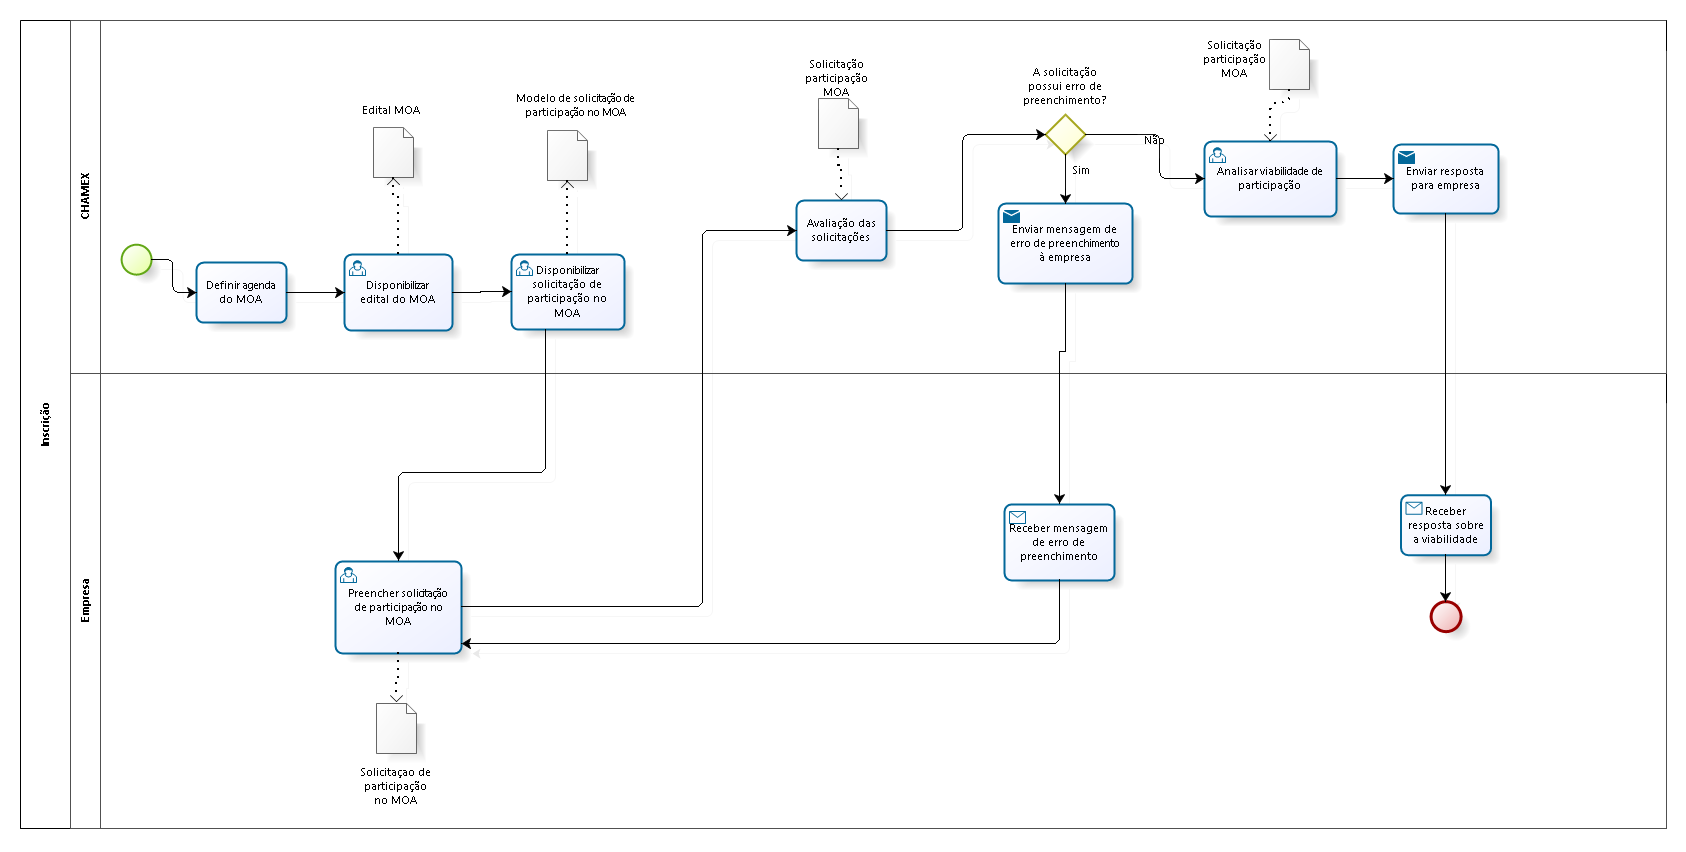
\includegraphics[scale=0.55]{inscricao_moa}
		\caption[Processo de Inscrição no MOA]{Processo de Inscrição no MOA.}
		\label{fig:processo_inscricao}
	\end{figure}
	\vspace*{\fill}
\end{landscape}